\section{Introduction}
\label{sec:intro}


% Architectures:
% - blues: Intel x86 cluster, fast Internet bandwidth
% - disco: Intel x86_64 cluster, slow Internet bandwidth
% Application characteristics
% - Workflow = loops of interleaved computation + communication
%   - In the loop: computation => communication => computation => communication ...
% - The computation hardware is idle when doing communication
% - Computation bound / communication bound
%
As computing platforms migrate toward clusters of heterogeneous processors connected by varying
network capacities, applications often need to manage the distributed memories of the processors
via explicit message-passing runtimes, for example, MPI.
Since the latency and bandwidth of the communication network are often hard to predict a priori, application performance is
often critically determined by the ability to flexibly overlap communications with local computations, thereby minimizing
wait time.

To illustrate the optimization, Figure~\ref{fig:ft_loop} shows the structure of the NAS FT benchmark~\cite{npb},
  which applies fast Fourier transform (FFT) to a 3D matrix through a loop that interleaves the computation of scaling  the input matrix
with a collective communication of MPI\_Alltoall to exchange data among the processes. This is then followed by a final transposition
of the resulting matrix.
The clear separation of computation and communication phases makes the algorithm design easy to implement and maintain.
Additionally, the communication buffers can be reused across different loop iterations, saving memory.
However, the blocking MPI communication requires that all processes wait while the MPI\_Alltoall operation is in progress.
Consequently, unless the application is executed on a platform with the fastest network connections, its performance is likely to suffer
because of the excessive wait time.

% https://en.wikibooks.org/wiki/LaTeX/Floats,_Figures_and_Captions
\begin{figure}
  \centering
  \begin{subfigure}[b]{0.2\textwidth}
    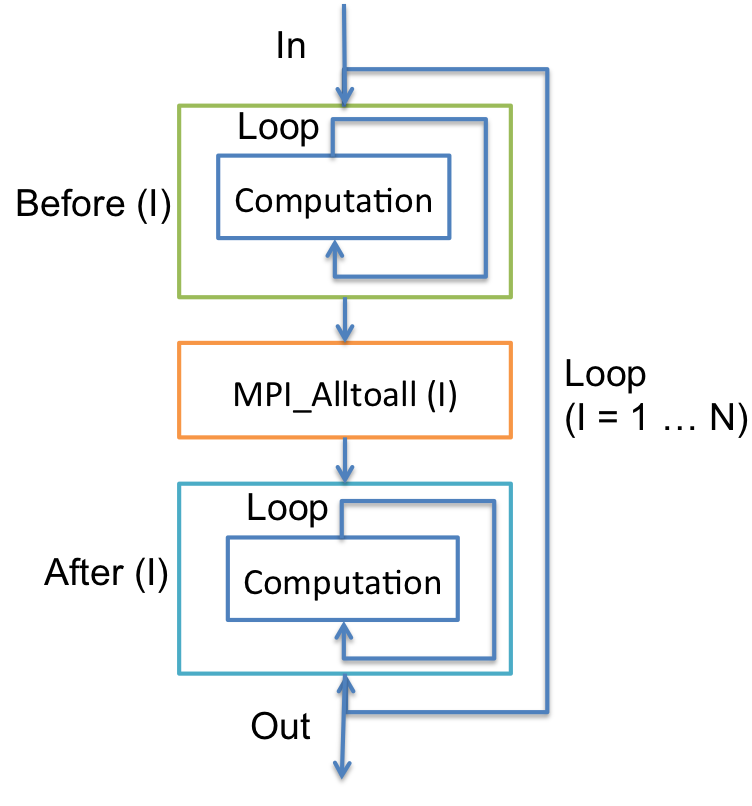
\includegraphics[width=0.8\textwidth,height=1.8in]{fig/ft_loop.png}
    \caption{Before optimization}
    %\caption{Loop with iterative computation and communication}
    \label{fig:ft_loop}
  \end{subfigure}%
  %add desired spacing between images, e. g. ~, \quad, \qquad, \hfill etc.
  %(or a blank line to force the subfigure onto a new line)
  \hspace{-.3in}
  \begin{subfigure}[b]{0.3\textwidth}
    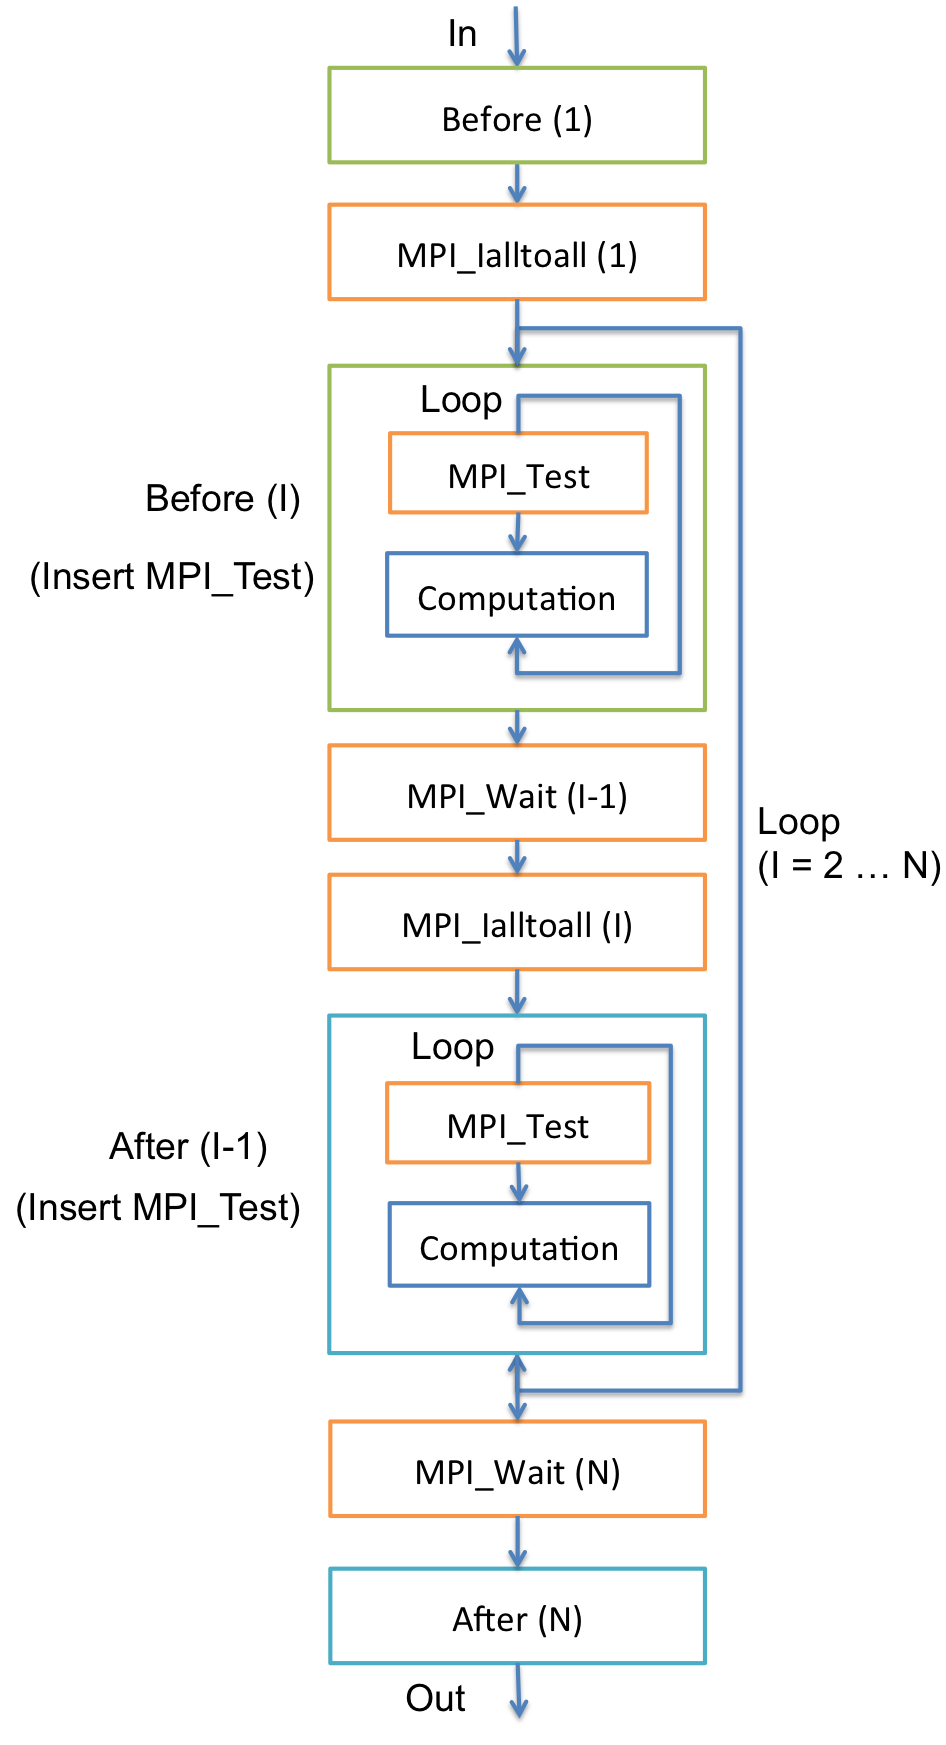
\includegraphics[width=1.1\textwidth,height=1.8in]{fig/ft_cco.png}
    \caption{After optimization}
    %\caption{Decouple and overlap the communication of the i-th iteration with the computation of the (i-1)-th and (i+1)-th iterations}
    \label{fig:ft_cco}
  \end{subfigure}
  \caption{Structure of NAS FT (1D layout) before (a) and after (b) overlapping computation and communication.
           \emph{Before} and \emph{After} in the figures are computation loops before and after the communication.}
\label{fig:ft}
\end{figure}

Figure~\ref{fig:ft_cco} illustrates how the structure in~\ref{fig:ft_loop} may be modified to better overlap computation with communication.
In particular,
   the MPI\_Alltoall operation is decoupled into two finer-grained operations: a nonblocking MPI\_Ialltoall and a blocking MPI\_Wait.
Then, the loop is modified so that Before(i), which multiplies a local matrix with a time-evolution array and then saves a transpose of the matrix into a local buffer to be communicated to other processors,  and MPI\_Ialltoall(i),  which exchange the local transposes among different processes, 
 are essentially moved so that they are evaluated before $MPI\_Wait(i-1)$, which waits for the completion of MPI communication of the previous iteration, and $After(i-1)$, which processes the just received remote data (of the $i-1$th iteration), and then print the result into an output file. 
By using two distinct buffers to store the data used in consecutive MPI communications,  the output dependencoes between After(i-1) and Before(i)/MPI\_Ialltoall(i) can be
eliminated, thereby guaranteeing the safety of optimization.

   \emph{MPI\_Test} operations are inserted into the local computation to ensure the progress of the nonblocking communications.\footnote{
  Although MPI communications do not need full usage of CPU, they need some CPU time,
 e.g., to manage communication buffers,
which is supplied only when operations such as MPI\_Test and MPI\_wait are invoked.}
By overlapping the MPI communications with the local computations, the transformed code
allows the application to perform well even on systems with slow network connections, although
nonblocking communications generally take longer time to finish than blocking ones,
and more memory may be needed to hold the data during communications.

\begin{figure}[h]
\centering
%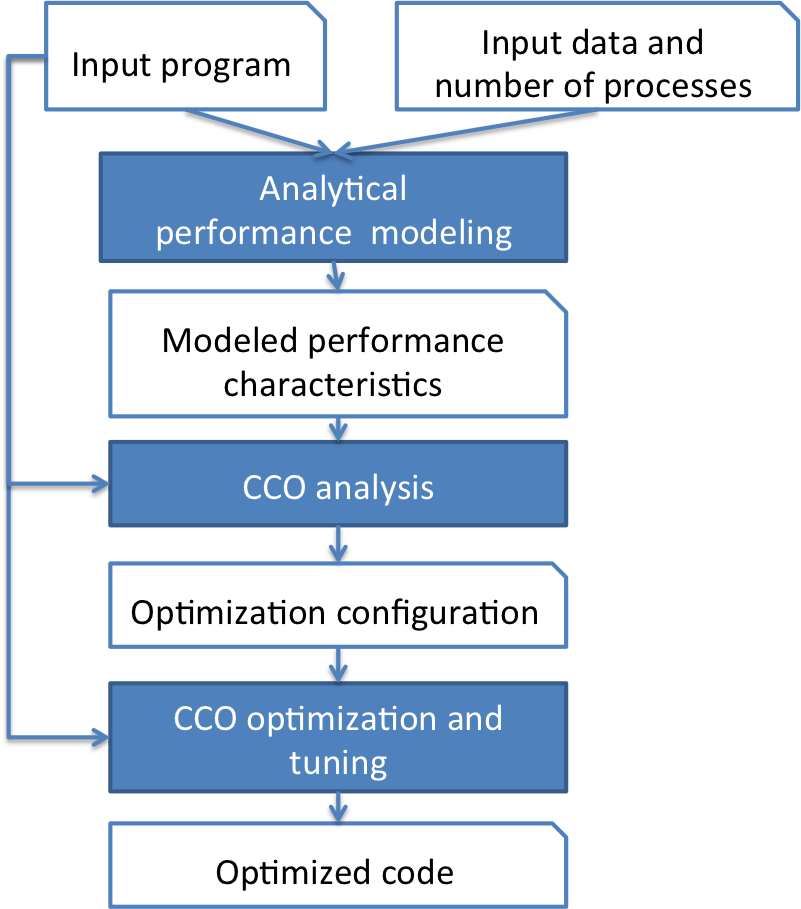
\includegraphics[width=0.48\textwidth]{fig/framework.png} % half page
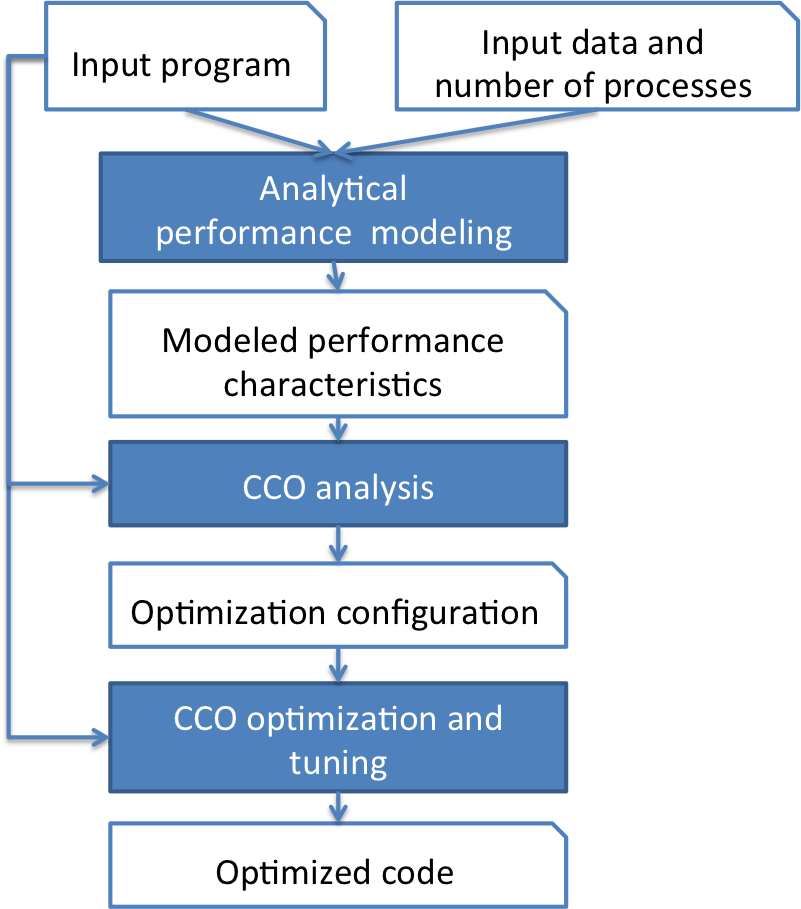
\includegraphics[width=0.35\textwidth]{fig/framework.png} % half page
\caption{Workflow of the CCO optimization approach}
%The components in the dashed box is extended from our SKOPE framework~\cite{jichi:ipdps14}.
\label{fig:overview}
\end{figure}

Figure~\ref{fig:overview} shows our workflow for systematically enabling communication-computation overlapping (CCO) in large MPI
applications and thereby enhancing their performance portability.
The workflow contains three key components:  (1) the \emph{performance modeling} component,
which analyzes the runtime statistics of an MPI application to extract a {\emph Bayesian execution tree\cite{jichi:ipdps14}} representation of
its execution flow, including the frequencies of various runtime code paths and their performance characteristics such as computation intensities,
working set sizes, and  communication characteristics of MPI operations;
(2) the \emph{CCO analysis} component, which identifies {\emph hot} computation and communication regions
 that are likely to benefit from the optimization and  summarizes the result of profitability and safety analysis of the optimizations;
and (3) the \emph{CCO optimization and tuning} component, which applies the appropriate program transformations by replacing the blocking MPI operations with
nonblocking ones, by reordering the computations and communications involved and
  by inserting MPI\_Test operations with a frequency determined by empirical tuning of the optimized code.
Note that in order to guarantee the profitability of the optimization,
any communication slowdown from the use of the nonblocking operations must be fully overlapped with the local computation,
and the insertion of MPI\_Test operations should cause only marginal slowdown of the local computation so that its effect is
insignificant when compared with the reduction of the original communication time.
Our framework currently uses empirical tuning of the optimized code to select appropriate optimization configurations and to skip nonprofitable optimizations.
%The computation intensity is represented by the numbers of fixed-point and floating-point instructions.
%The memory accesses include the allocated memory sizes and numbers of loads and stores.
%The communication behaviors consist of the MPI functions being invoked,
%    and the runtime parameters of data types and transferred data sizes.
%    and identifies top time-consuming communication and computation hot spots
%    as the MPI function calls having the largest communication cost, or the basic blocks takes the largest computation time.
%Then, the computation and communication time for each code path is projected from the performance characteristics
%  using Roofline\cite{roofline} and LogGP\cite{loggp} models.
%in MPICH 3.1, MPI\_Alltoall and MPI\_Ialltoall are implemented using different algorithms that
% MPI\_Alltoall can benefit from the hardware support for collective operation,
% while MPI\_Ialltoall is implemented as non-blocking send/recv and do not have such benefit.
%and the MPI\_Test operations, when inserted too frequently, can slowdown the computations.
%  it might require at most two times of the memory to hold the buffer for two iterations.
%Finally, when the communication or computation to overlap takes short time,
%  the overlap speed up might not be large enough to overcome the above slowdown.

Our main contributions are the following:
\begin{itemize}
 \item We present a framework that integrates analytical performance modeling of large MPI applications, semantic inlining of developer-supplied domain knowledge, and pattern-based transformation in order to systematically enable better overlapping of MPI communications with independent local computations to enhance the performance portability of MPI applications. We currently manually applied the necessary program transformations (the last stage of the optimization) but expect to automate this step in our future work. 
  \item We applied our approach to optimize 7 NAS Parallel Benchmarks (NPB) applications on both a high-speed and a slow network-connected cluster environment and achieved 3--88\% speedup on both platforms.
\end{itemize}


The remainder of the paper is organized as follows.
Section~\ref{sec-model} presents our analytical performance modeling component for automatically identifying communication and computation hot spots in MPI applications
Section~\ref{sec-analysis} discusses how to determine the safety of computation-communication overlap through optimization analysis.
Section~\ref{sec-opt} summarizes strategies we used to perform the actual optimizations and the tuning of their configurations.
Section~\ref{sec-exp} evaluates our framework using 9 NAS application benchmarks~\cite{npb}.
Section~\ref{sec-related} discusses related work, and
Section~\ref{sec-concl} presents our conclusions.

% EOF

%and tuning the frequency on the target runtime environment using simple binary search.
  %we manually decouple the blocking communication into non-blocking functions
  %and reorder them in the parent loop so that the communication in the current iteration can overlap with the computation from previous and next iterations.
%The frequency of MPI\_Test is parameterized for each loop for overlapping.
%The frequency of MPI\_Test is tuned using binary search on the target platform.
%The places of MPI\_Test are selected so that the computation time between two MPI\_Tests are roughly the same.
%The total number of MPI\_Tests are tuned for the target input data and runtime environment.
%As the communication polling frequency is dependent on the load-balance of the communication and computation time at runtime,
%  we tune it using binary search for different input data and runtime parameters.
%The framework takes the source code, input data of the application, and the runtime MPI process number as input,
%  and output optimization hints that summarize
%     the inter-procedural structure of computation and communication to overlap as well as the places to insert MPI\_Test.
%Our approach essentially uses an analytical modeling approach
%  to analyze application's runtime code path and project execution time
%  to identify potential communication and computation hot spots.
%The hot spots are then used to select candidate loops to apply CCO optimization,
%  and the modeled execution time is used to select where MPI\_Test should be inserted.
%The overall workflow of our approach includes three steps as shown in Figure~\ref{fig:overview}.

%\begin{figure}
%\centering
%{\scriptsize
%  \begin{subfigure}[b]{0.24\textwidth}
%\begin{verbatim}
%MPI_Ialltoall
%Loop I = 1 ... L
%  If I % Freq == 0
%    MPI_Test
%  Computation
%MPI_Wait
%\end{verbatim}
%  \caption{Single computation loop}
%  \label{fig:cco_test:single}
%  \end{subfigure}%
%  \begin{subfigure}[b]{0.24\textwidth}
%\begin{verbatim}
%MPI_Ialltoall
%Loop I = 1 ... L1
%  If I % Freq1 == 0
%    MPI_Test
%  Computation1
%Loop I = 1 ... L2
%  If I % Freq2 == 0
%    MPI_Test
%  Computation2
%...
%Loop I = 1 ... LN
%  If I % FreqN == 0
%    MPI_Test
%  ComputationN
%MPI_Wait
%\end{verbatim}
%  \caption{Multiple computation loops}
%  \label{fig:cco_test:multiple}
%  \end{subfigure}%
%\caption{Single or multiple computation loops with MPI\_Test inserted}
%\label{fig:cco_test}
%}%\scriptsize
%\end{figure}

%\begin{figure}
%{\scriptsize
%\begin{verbatim}
%for 6:
% evolve():
%   for 256: for 256: for 512: MPI_Test(0.09)
% fft():
%   cffts1():
%     for 256: for 512:
%       cfftz(): for 16:
%         fftz2(): for 512: MPI_Test(0.14)
%         fftz2(): for 512: MPI_Test(0.14)
%   transpose_x_yz():
%     transpose2_local()
%     transpose2_global(): for 16: for 32768: MPI_Test(0.08)
%       mpi_alltoall():
%     transpose2_finish(): for 16: for 32768: MPI_Test(0.07)
%   cffts2():
%     for 256: for 512:
%       cfftz(): for 16:
%         fftz2(): for 512: MPI_Test(0.11)
%         fftz2(): for 512: MPI_Test(0.11)
%   cffts1():
%     for 256: for 512:
%       cfftz(): for 16:
%         fftz2(): for 512: MPI_Test(0.13)
%         fftz2(): for 512: MPI_Test(0.13)
%\end{verbatim}
%\caption{Distribution of MPI\_Test inserted into the overlapped computation}
%\label{fig:ft_output}
%}%\scriptsize
%\end{figure}

%The computation-communication-overlap (\textit{CCO}) optimization
%  can make usage of the idle computation hardware during the communication
%  by reordering the communication and computation
%  to reduce the overall runtime from the $sum$ to the $maximum$ of the computation and communication time.
%In short, the computation-communication-overlap (\textit{CCO}) optimization
%  %can make usage of the idle computation hardware during the communication
%  %by reordering the communication and computation
%  can reduce the overall runtime from the $sum$ to the $maximum$ of the computation and communication time.
%A common strategy to overlap computation and communication can be divided in to three steps:
%  first, find the critical path of the application;
%  then, decouple the communication to the non-blocking version, and reorder the computation and computation to overlap;
%  and finally, insert MPI\_Test into the computation to dynamically adjust the communication frequency.
%In particular, the most time-consuming communication is the MPI\_Alltoall in the main loop
%  that takes more than 60\% of the overall runtime.
%\begin{itemize}
%\item % Portability
%The CCO optimization highly depends on the runtime hot paths of the application.
%As the critical path and hot spots for distributed memory application are runtime-dependent,
%The critical path and hot spots are runtime dependent on the input, hardware, and runtime environment.
%As the critical path and hot spots for distributed memory application are runtime-dependent,
%In NAS FT,
%   the critical path is different by whether 0D, 1D or 2D layout of the FFT transformation will be applied,
%   which is determined by the input parameters and the number of processes;
%and even on the same critical path,
%  the computation hot spots could vary
%  by different problem sizes and the underlying hardware.
%\item % Inter-procedural analysis and runtime code paths
% In NAS FT, the same communication hot spots is invoked both before and after the hot communication.
% My explanation here is weak ... as our framework cannot do safety analysis at the moment.
%\item
%Third, the communication and computation are
%  usually spread in different procedures,
%  which increase the challenge to extract the high-level computation structure.
%\end{itemize}


%And the overall performance
%  is bounded by the sum of the total computation and communication time on the critical path.
% Advantage of CCO: sum(communication, computation) => max(communication, computation)

%\todo {This is not what I meant by discussion of example. You need to actually show the code or its structure/workflow, analyze the code, to show what you exactly mean}
% Example: NAS FT
% Workflow:
% - Loop
%   - Local transpose
%   - Global alltoall
%   - Local transpose
%For example, NAS FT is a well-known communication-bound application
%  that applies FFT transformation to 3D matrices.
%The critical path of NAS FT is composed of iterations of
%   matrix transposition computation and alltoall communication,
%   and the communication time usually takes more than half of the overall runtime
%     depending on the runtime environment.
%A common way to overlap the alltoall communication with the computation can be done using the following steps:
%\begin{enumerate}
%\item Find the most time-consuming MPI\_Alltoall communication to overlap.
%\item Decouple the MPI\_Alltoall to non-blocking MPI\_Ialltoall and MPI\_Wait.
%\item Reorder the iterations of communication and computation
%      by moving the computation from previous and next iterations
%      into the middle of MPI\_Ialltoall and MPI\_Wait in the current iteration.
%\item Insert MPI\_Test into the overlapped communication to dynamically adjust the communication frequency.
%\end{enumerate}
%\done{Now talk about what are the key challenges of performing cco}
%While the MPI standard provides non-blocking APIs for overlapping,
%  it relies on the developers for the performance and portability of the optimization.
%The challenges to properly apply steps are:
% - Portability
% - Interprocedural
% - MPI_Test frequency
%\begin{itemize}
%\item % Portability
%%The CCO optimization highly depends on the runtime hot paths of the application.
%The critical path and hot spots are runtime dependent on the input, hardware, and runtime environment.
%%As the critical path and hot spots for distributed memory application are runtime-dependent,
%In NAS FT,
%   the critical path is different by whether 0D, 1D or 2D layout of the FFT transformation will be applied,
%   which is determined by the input parameters and the number of processes;
%and even on the same critical path,
%  the computation hot spots could vary
%  by different problem sizes and the underlying hardware.
%\item % Inter-procedural analysis and runtime code paths
%The communication and computation hot spots are
%  usually spread in different procedures,
%  which increase the challenge to extract the runtime critical path.
%% In NAS FT, the same communication hot spots is invoked both before and after the hot communication.
%% My explanation here is weak ... as our framework cannot do safety analysis at the moment.
%\item The MPI\_Test frequency in the computation loop is runtime-dependent on the load-balance of the communication and computation time.
%When the frequency is small, the background communication might not have enough polls to finished.
%However, when the frequency is large, it might slowdown the computation loops.
%When there are multiple computation hot spots to overlap,
%  the problem to select MPI\_Test frequency will become more challenging
%  that requires runtime knowledge about the computation and communication time for each hot spot.
%  %because MPI\_Test should be ideally evenly distributed in the overlapped computation,
%  %the selection of frequencies would require the knowledge of the runtime computation time of the hot spots,
%\end{itemize}

%The performance of distributed memory applications
%  is determined by both the computation and communication
%  distributed over the cluster with runtime-dependent communication bandwidth and number of processes.
%The critical path to performance
%  is usually made from iterations of interleaved communication and computation hot spots,
%%Depending on network bandwidth and the load-balance of processes,
%%  the communication could take even more time than the computation.
%%Given fixed memory and network architecture,
%  and the overall performance is bound by how much computation and communication can be overlapped.
%%MPI applications generally manage large amounts of data and heavy computation
%%distributed over the cluster with runtime-dependent communication bandwidth and number of processes.
%%A common problem of these applications is that
%%  the underlying computation hardware has to wait idly
%%These applications commonly have the problem of
%%  waiting idly in the middle of the computation
%%  for the communication to finish exchanging data with other nodes.
%%One of the key problems for optimization
%%  is to select the most time-consuming computation and communication code regions
%%  and overlap them to make full use of the idle hardware.
%%The first step in the overlapping optimization is usually to select the hot computation and communication to overlap.
%%As the communication and computation hot spots are runtime-dependent on
%%  the input data, underlying hardware, and the runtime network topology such as the number of processes,
%%%To select the computation and communication to overlap,
%%  the application usually has to be re-profiled repeatedly
%%  whenever the input or the runtime parameters are changed. %parameters such as the number of processes or input data sizes are changed.
%%While MPI standard provides non-blocking functionality to support overlapping,
%%  it relies on the developers to achieve good performance over variant runtime environment.
%% II. Elaborate Challenges
%% Main challenges
%% - Easily to find computation and communication for variant hardware
%% - Inter-process
%The overlapping optimization generally can be divided into three steps.
%First, profile the application to identify the communication and/or communication hot spots;
%second, select the code block containing the hot computation and communication to overlap;
%and third, decouple the hot communication into non-blocking functions
%  and interleave them with the hot computation.
%When the communication and the computation hot spots
%  are scattered in different procedures that is usually the case,
%  it would increase the complexity for developers to select the proper overlapping code block for large applications
%  that could consist of thousands of procedures.
%Additionally, the communication and computation hot spots
%  are usually runtime-dependent on the input data, network topology, and the underlying architectures
%  that are not portable.
%As the results,
%  developers usually have to manually repeat the three steps to get the optimal performance for different runtime environment.

% III. My Approach

%% Motivate computation communication overlap
%MPI is a de facto standard for distributed computing
%of large-scale scientific applications.
%MPI applications spend time on both computation and communication,
%which creates an optimization opportunities
%to overlap computation and communication.
%%% Challenges to overlap computation and communication manually
%However, it is challenging to have an optimal overlap implementation
%to out-perform on all variant runtime environment.
%%But it is challenging is to identify proper overlappable communication and computation workflow.
%To select proper computation and communication code regions to overlap,
%the input data sizes, number of processes, and the network topology of the network topology
%are needed, %estimating the computation and communication time,
%which could be both input- and hardware-dependent.
%Additionally, it is also challenging for compilers to automatically apply the overlap optimization
%for each runtime environment.
%The deeply-nested function calls and the absence of input data and communication pattern
%increase the difficulties for accurate offline dependence analysis,
%which is indispensable for checking the safety of the overlap transformation.
%As a result, developers usually have to profile the applications for various input and the target platform,
%and manually apply the optimizations.

%The framework essentially used the previous approaches of annotation-based inlining and analytical modeling to address the challenges.
%The annotation-based inlining is used to help reduce the complexity of the deep-nested inlined code
%as well as providing programming interface for the developer to specify the runtime code path of the inlined functions.
%The analytical modeling approach was used to (1) integrate hardware model and profiling to estimate communication bottlenecks,
%as well as (2) perform course-grained whole-program analysis to find small optimization scope.
%Both of the two approaches are used to integrate domain knowledge and reduce the code size for later fine-grained overlap optimization analysis.
%Our technique is built upon previously proposed modeling techniques.

%It takes the application's source code as well as the profiling results and hardware models,
%and generates the source code optimized for the target runtime environment.
%The workflow that can be divided into the following four stages:
%\begin{enumerate}
%\item Hardware calibration to get the parameters for the computation and communication hardware performance models.
%  The hardware performance models are used to analytically estimate computation and communication time for a workflow.
%  The roofline model is used to model computation.
%  And I developed a profiling-based communication model for estimating balanced MPI two-sided and collective communication time.
%\item Skeleton-based modeling for course-grained analysis to find hot communication and candidate overlap code regions.
%  First, an analytical execution-flow model will be constructed for the application.
%  Then, combining with hardware models, the hot region analysis will be applied to find hot communication.
%  %First, generate skeletons from the source code to construct an execution flow model.
%  %Then, select a few top hot communication spots by the hot region analysis.
%  And finally,
%  an inter-procedural analysis will be applied on the execution-flow model
%  to compute the candidate overlap region that might contain overlappable hot communication and computation.
%\item Optimization analysis to compute overlappable computation in the estimated overlap code region.
%  Given the hot communication and the enclosing overlap region,
%  the optimization analysis will first apply annotation-based inlining to erase the procedure boundaries,
%  and then
%  %The first step is to use annotation-based inlining to help erase the procedure boundaries.
%  use data dependence analysis and control flow analysis to find
%  the computation that are either independent from the communication, or can be decomposed to interweave with the communication.
%%\item Program transformation to generate the optimized code for the target hardware.
%%  %Generating CCO pragmas
%%  % Transform the code
%\end{enumerate}
%that can be divided into four stages, as follows:

%The rest of this chapter is organized as follows.
%Section~\ref{sec:exeflow} will discuss the performance models and execution flow modeling used in the framework.
%Section~\ref{sec:hot} will discuss the analytical analysis to find computation and communication hot spots.
%Section~\ref{sec:pragma} will discuss the course-grained analysis to generate optimization directives from BET.
%Section~\ref{sec:inline} will discuss the inter-procedural analysis to generate parameterized pragmas with annotation-based inlining.
%Section~\ref{sec:tune} will discuss the program transformation for generating the optimized source code.
%%Section~\ref{sec:mpi:tr} will shows the program transformation process.
%And at last, Section~\ref{sec:exp} will presents the experimental results. % on the effectiveness of the new approach,

%The framework is overall an analytical optimization analyzer which takes the input source code
%  and the performance models, %and the domain knowledge from developers,
%  and suggests computation and communication code regions that can be potentially overlapped.

%For large-scientific applications, there are two main challenges to find overlappable computation and communication:
%\begin{enumerate}
%\item The large code base and nested function calls would increase the complexity of inter-procedural analysis.
%\item The overlappable computation and communication regions could be runtime-dependent
%on the input data, code path, and network bandwidth.
%Domain-knowledge about the application's runtime behaviors and the underlying platform becomes indispensable.
%\end{enumerate}
%To address these challenges, I especially used my previous technique of annotation-based inlining and analytical modeling.
%The annotation-based inlining is used to help reduce the complexity of the deep-nested inlined code
%as well as providing programming interface for the developer to specify the runtime code path of the inlined functions.
%The analytical modeling technique was used to (1) integrate hardware model and profiling to estimate communication bottlenecks,
%as well as (2) perform course-grained whole-program analysis to find small optimization scope.
%Both of the two techniques are used to integrate domain knowledge and reduce the code size for later fine-grained overlap optimization analysis.

%The framework is built on top of my existing work on analytical execution-flow modeling and annotation-based inlining,
%which are extended in the following directions:
%\begin{itemize}
%\item Analytical modeling
%  \begin{enumerate}
%  \item Add a profile-based communication model based on LogP model for roughly estimate MPI point-to-point and collective communication time.
%  \item Add execution-flow analysis to find hot communication and the overlap code region.
%  \end{enumerate}
%\item Annotation-based inlining
%  \begin{enumerate}
%  \item The annotation can be automatically generated from the source code.
%        Comparing to the conventional inlining, computation details are skipped in the inlined code
%        to reduce the complexity for later analysis.
%  \item The inlining was for program analysis than program transformation.
%        The inlined nodes in the AST was tracked by the line numbers of the original code that generate the annotation.
%  \end{enumerate}
%\end{itemize}

%The rest of this chapter is organized as follows.
%Section~\ref{sec:mpi:commmodel} will show the communication model used in our framework.
%Section~\ref{sec:mpi:hotcomm} will discuss the analytical analysis to find hot communication spots.
%Section~\ref{sec:mpi:hotregion} will describe the technique to estimate the overlap code regions.
%Section~\ref{sec:mpi:inline} will discuss the annotation-based inlining transformation.
%Section~\ref{sec:mpi:cco} will introduce the algorithms to compute the independent and decomposable computation.
%%Section~\ref{sec:mpi:tr} will shows the program transformation process.
%And at last, Section~\ref{sec:mpi:exp} will presents the experimental results. % on the effectiveness of the new approach,

%The optimization analysis could be divided into four stages:
%\begin{itemize}
%\item Hotspot analysis.
%It utilizes the performance model and profiling to find the hot communication to optimize.
%The output is either a single communication statement or a group of decoupled communication.
%The purpose is to reduce the amount of code to optimize for large applications.
%\item Compute the overlap code region.
%It takes the hot communication from the hotspot analysis,
%  and output a code region where the computation in it could be overlapped with the communication.
%The analysis only does control flow analysis.
%The portability analysis which varies by different hardware is not applied.
%\item Inline functions.
%After the overlap region is selected, the inlining stage use annotation-based inlining
%  to break the procedural boundaries of the scope to reduce the complexity for later optimizations.
%The annotation is automatically generated to expresses only the control flow and the data dependence while ignoring the computation details.
%\item Compute independent and decomposable workflows.
%After the inlining stage, there will be a code region where intra-procedural dependence analysis can be applied.
%This stage will build a dependence group to find the candidate computation that are either independent
%  from the communication, or can be decomposed in the same way as the communication.
%\item Generate CCO pragmas
%The overlap region, hot communication, independent and decomposable workflows from the previous stages
%  are encoded into CCO transformation pragmas inserted to the source code.
%\end{itemize}

% - Use performance model to find hot communication and communication path
% - Use BET to apply inter-procedural analysis
% - Tuning MPI_Test frequencies
%   Single computation hot spots: binary search
%   Multiple computation hot spots:
%       Assumption, MPI_Test should be evenly distributed in the computation.
%       frequencies are based on the ratio of different computation hot spot performance
%          given: (time1 / loop1) * count1 =  time2 / loop2 * count2 = time3 / loop3 * count3
%          so, count1 : count2 : count3 = loop1/time1 : loop2 / time2 : loop3 / time3
%       If count < 1 do not insert MPI\_Test
%       Binary search to all counts

%Our experimental results show that when MPI\_Test frequencies in NAS FT could result in up to \todo{how much} difference to the overall performance
%  using \todo{how many} nodes,
%and the best performance is achieved when the minimum number of MPI\_Test is evenly distributed in the overlapped computation time.

%As shown in Figure~\ref{fig:cco_test:single}, when there is only one computation loop to overlap,
%  MPI\_Test can be inserted to the beginning of the loop,
%  and the optimal frequency $Freq$ for the target runtime environment can be tuned using binary search.
%But when there are multiple computation loops to overlap as shown in Figure~\ref{fig:cco_test:multiple},
%  which is common in NAS Parallel Benchmark,
%  finding the optimal combination of $Freq1 \ldots FreqN$ becomes a challenging problem.

%One the other hand, the MPI\_Test frequencies in the computation loops are runtime-dependent on the load-balance of the communication and computation time.
%When the frequency is small, the background communication might not have enough polls to finished.
%However, when the frequency is large, it might slowdown the computation loops.
%The problem to insert MPI\_Test would become more complicated when there are multiple computation hot spots to overlap
%  %because MPI\_Test should be ideally evenly distributed in the overlapped computation,
%  that requires the knowledge of the runtime computation time of these hot spots,

%While the MPI standard provides non-blocking functionality,
%  it relies on the developers to handle the challenges for the performance and portability of the optimization.
%On one hand, the same application could have different hot computation and communication
%  that is determined by the input data, underlying hardware, and runtime environment such as the number of processes.

% See: mpich-3.1.1/src/mpid/ch3/channels/nemesis/src/ch3_progress.c
% There are for kinds of progress beyond prepare/complete a request
% - prepare the request
% - make progress receiving
% - make progress sending
% - make progress on LMTs (Large Message Transfer)
% - make progress on NBC schedules: non-blocking communication
% - complete the request

%On the other hand, the inserted MPI\_Test ideally should be \emph{evenly distributed} in the overlapped computation time
%  to periodically make progress in the communication,
%  and the communication should \emph{just} finish at the same time as the computation
%    with minimum number of MPI\_Test.
%% 1. Computation time in between MPI\_Test are equal.
%% 2. Communication is just finished before MPI_Wait.
%% 3. Minimum MPI_Test.
%An example runtime code path of the overlapped computation with inserted MPI\_Test is shown in Figure~\ref{fig:cco_test}.
%When evenly-distributed,
%  the computation time between each two MPI\_Test is roughly equal.
%The total number of MPI\_Test should be the smallest when the communication just finishes before MPI\_Wait that can be safely removed.
